% ============================================================
%  Temporal Partial Information Decomposition of EEG During Sleep
%  1-second window pass — Technical Report
%  Mirrors structure of pid_sleep_report.tex (30-s pass);
%  compile with pdflatex.
% ============================================================
\documentclass[11pt,a4paper]{article}

\usepackage[margin=2.5cm]{geometry}
\usepackage{amsmath,amssymb}
\usepackage{graphicx}
\usepackage{booktabs}
\usepackage{array}
\usepackage{caption}
\usepackage{subcaption}
\usepackage[colorlinks=true,linkcolor=blue,citecolor=blue,urlcolor=blue]{hyperref}
\usepackage{microtype}
\usepackage{xurl}
\usepackage{parskip}
\usepackage{xcolor}
\usepackage{siunitx}

\usepackage{natbib}
\bibliographystyle{plainnat}

\title{\textbf{Temporal Partial Information Decomposition\\of Human EEG Across Sleep Stages}\\[4pt]
\large Short-window pass (1-second resolution)}
\author{Temporal Information Decomposition Project}
\date{June 2026}

% ============================================================
\begin{document}
\maketitle
\tableofcontents
\newpage

% ============================================================
\section{Abstract}
% ============================================================

We re-apply \emph{Temporal Partial Information Decomposition} (Temporal PID) to
overnight polysomnography EEG from 10 healthy adults using a \textbf{1-second
window} configuration that brings the analysis into a temporal scale appropriate
for EEG dynamics.  For every 1-second EEG window we construct temporal triplets
at pairs of second-scale lags ($\tau_1, \tau_2 \in [1, 30]$~s) and decompose the
predictive information about the target window into four atoms ---
\emph{redundancy}, \emph{synergy}, \emph{unique information from the shorter
lag} (Unique$_1$), and \emph{unique information from the longer lag}
(Unique$_2$) --- using the Minimum Mutual Information (MMI) PID measure,
implemented in closed form (verified to $10^{-15}$ against the \texttt{dit}
reference).  The first 3.5 hours of each recording are analysed --- enough for
two NREM--REM cycles plus per-stage AR(1) fits.

This pass updates the 30-second report in three substantive ways.  First, the
block-permutation null now shuffles 1-second blocks, destroying nearly all
linear autocorrelation at the tested lag scales rather than preserving it.
Second, the AR(1) baseline is \textbf{stage-conditional}: $\phi$ and $\sigma$
are fit per sleep stage on that stage's windows alone, isolating non-linear
excess from across-stage spectral differences.  Third, a new figure (the
per-stage PID excess + double-dissociation strip) directly addresses the
question of whether stages differ in \emph{how} they exceed their own linear
baseline, not just by how much.

% ============================================================
\section{Introduction}
% ============================================================

Sleep staging traditionally rests on spectral features such as slow-wave power,
sleep spindle density, and K-complex count~\citep{berry2012aasm}.
These measures capture \emph{linear, single-timescale} properties of the EEG.
The rich temporal dynamics of sleep --- travelling slow oscillations that
coordinate memory consolidation, hippocampal sharp-wave ripples, and
thalamo-cortical spindles --- involve \emph{multi-timescale, non-linear}
interactions that spectral power alone cannot resolve.

Partial Information Decomposition (PID)~\citep{williams2010nonnegative} is an
information-theoretic framework that decomposes the total predictive
information shared between a set of source variables and a target into
non-negative, non-overlapping atoms: information carried \emph{redundantly} by
all sources, information \emph{unique} to each source, and information
available only when sources are considered \emph{jointly} (synergy).
When applied across temporal lags (comparing a signal to its own past at two
different delays), PID quantifies the temporal self-predictability structure of
neural dynamics.

The companion 30-s pass~(\citet{pid_sleep_report_30s}) established that all four
PID atoms vary highly significantly across sleep stages on this dataset.  Two
methodological concerns motivated the present short-window pass.  First, a
30-second block is long for EEG --- the EEG meaningfully changes within a
30-second window, and a 30-second block-permutation null preserves nearly all
the temporal structure of interest, weakening the null's informativeness.
Second, the global (non-stage-conditional) AR(1) baseline used previously
confounds within-stage non-linear excess with across-stage spectral
differences.  Both are addressed here.

% ============================================================
\section{Methods}
% ============================================================

\subsection{Dataset and participants}

EEG data were taken from OpenNeuro \texttt{ds005555} (10 healthy adults,
overnight polysomnography).  The first 3.5~hours of each recording were
analysed --- a reduction from 5~hours that still captures two full NREM--REM
cycles while bounding wall-time at the 1-second resolution.  Six scalp channels
(F3, F4, C3, C4, O1, O2) were loaded with MNE-Python~\citep{gramfort2013meg};
sleep stages were read from the accompanying \texttt{*psg\_events.tsv} files
(AASM five-class system).

Figure~\ref{fig:method} provides an overview of the full pipeline; only the
window size, lag grid, and quantile-bin count differ from the 30-s pass.

\begin{figure}[tbp]
  \centering
  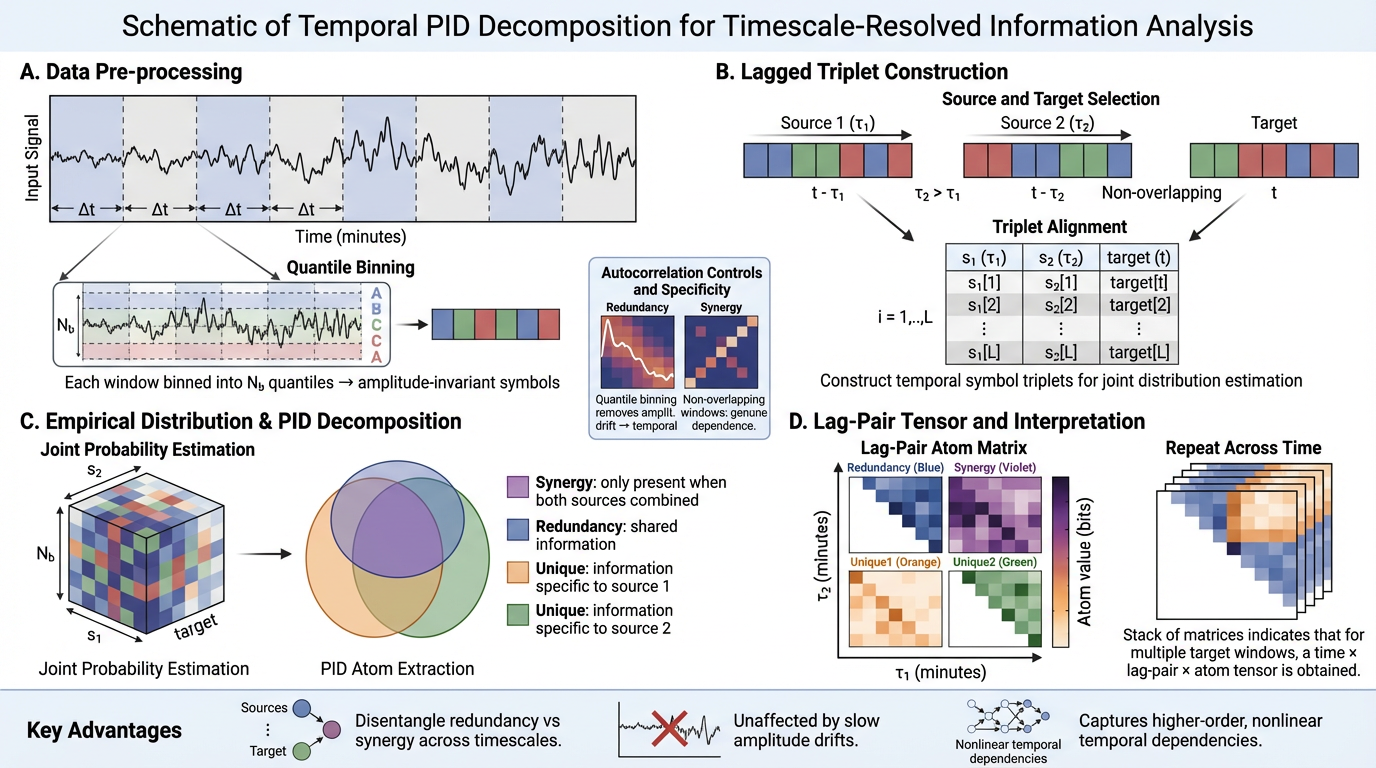
\includegraphics[width=\textwidth]{../docs/Temporal-PID_figure.png}
  \caption{%
    \textbf{Overview of the Temporal PID pipeline.}
    (A)~Input signal segmented into fixed-length windows
    ($\Delta t = 1$~s in this pass) and independently discretised into
    $N_b = 4$ quantile bins, producing amplitude-invariant symbol sequences.
    (B)~Lagged triplet construction: for each target window $t$, two past
    windows at offsets $\tau_1 < \tau_2$ are aligned sample-by-sample to form
    the source--target triplet
    $(\mathbf{s}_1, \mathbf{s}_2, \mathbf{x}(t))$.
    (C)~The empirical joint distribution over the
    $N_b^3 = 64$ symbol states is estimated by co-occurrence counts; PID with
    the MMI measure decomposes it into four non-negative atoms (redundancy,
    synergy, unique$_1$, unique$_2$).  At this pass the atoms are computed in
    closed form directly from the joint counts ($\sim 10^3 \times$ faster per
    call than the \texttt{dit} reference, verified to $10^{-15}$).
    (D)~Repeating the decomposition across all 435 lag pairs
    $(\tau_1, \tau_2)$ and all valid target windows yields a
    time $\times$ lag-pair $\times$ atom tensor.
  }
  \label{fig:method}
\end{figure}

\subsection{Preprocessing}

Each EEG channel was:
\begin{enumerate}
  \item Bandpass filtered (0.5--60~Hz, 4th-order Butterworth, zero-phase);
  \item Notch filtered at 50~Hz and 60~Hz (IIR notch, $Q = 30$) to remove
        power-line interference.
\end{enumerate}

\subsection{Windowing and Discretisation}

The continuous signal was divided into non-overlapping windows of
$\Delta t = \SI{1}{\second}$ (reduced from 30~s in the original pass), yielding
$N_w = \lfloor T / \Delta t \rfloor = 12{,}600$ windows over the 3.5-hour analysis
window.  Each window was independently discretised into $N_b = 4$ levels using
quantile binning.  $N_b$ was reduced from 6 because each 1-s window contains
only $f_s \cdot \Delta t = 256$ samples to estimate the joint distribution
$p(\mathbf{s}_1, \mathbf{s}_2, \mathbf{x})$.  At $N_b = 6$ the joint has 216
cells and only $256 / 216 \approx 1.2$ samples per cell on average; at
$N_b = 4$ this becomes $256 / 64 = 4$ samples per cell, the regime where the
empirical estimator behaves reasonably.

Per-window discretisation renders the analysis amplitude-invariant
\emph{within a window} (each window has its own quantile edges) and removes
any DC offset or slow drift on the window timescale, so that
information-theoretic measures capture temporal \emph{pattern} rather than
amplitude covariation.

\subsection{Temporal Triplet Construction}

For a target window $\mathbf{x}(t)$ and two lag offsets $\tau_1 < \tau_2$
(in \textbf{seconds}), the temporal triplet is
\begin{equation}
  \bigl(\mathbf{s}_1,\, \mathbf{s}_2,\, \mathbf{x}(t)\bigr)
  = \bigl(\mathbf{x}(t - \tau_1),\, \mathbf{x}(t - \tau_2),\, \mathbf{x}(t)\bigr).
\end{equation}
Sample-by-sample alignment yields $L = \Delta t \times f_s = 256$
co-occurring symbol triples per triplet formation.
Lag offsets are set on a 1-second grid from 1 to 30~s
($\tau \in \{1, 2, \ldots, 30\}$~s), producing
$\binom{30}{2} = 435$ distinct lag pairs $(\tau_1, \tau_2)$ with
$\tau_1 < \tau_2$.

The time-resolved PID is evaluated on a strided target axis with
\texttt{TARGET\_STEP} $= 3$ (one estimate every 3~s).  Each estimate still
uses the full 1-second target + 1-second source windows; only the time-axis
density of estimates is thinned --- global PID and AR(1) baseline are
unaffected.

\subsection{PID Decomposition}

The empirical joint distribution $p(\mathbf{s}_1, \mathbf{s}_2, \mathbf{x})$
over $N_b^3 = 64$ states was estimated by a single \texttt{bincount} over the
flat triplet codes.  \emph{Partial Information Decomposition} with the
Minimum Mutual Information (MMI) measure~\citep{barrett2015exploration} was
then applied in closed form,
\begin{align}
  R &= \min\!\bigl(I(\mathbf{s}_1;\mathbf{x}),\, I(\mathbf{s}_2;\mathbf{x})\bigr), \\
  U_i &= I(\mathbf{s}_i;\mathbf{x}) - R, \\
  S &= I(\{\mathbf{s}_1,\mathbf{s}_2\};\mathbf{x})
      - I(\mathbf{s}_1;\mathbf{x}) - I(\mathbf{s}_2;\mathbf{x}) + R.
\end{align}
This direct formulation is mathematically equivalent to the \texttt{dit}
library's \texttt{PID\_MMI}~\citep{james2018dit}; we verified agreement to
$10^{-15}$ across IID, COPY, XOR, and AR-correlated test cases.  At
256-sample joints the closed form is $\sim 500$--$1500\times$ faster per call
than the dit reference, which made the full multi-subject pass feasible.

\begin{table}[h]
\centering
\caption{PID atoms and their temporal interpretation.}
\label{tab:atoms}
\begin{tabular}{@{}lp{9cm}@{}}
\toprule
\textbf{Atom} & \textbf{Temporal interpretation} \\
\midrule
Redundancy~$R$ & Predictive information about $\mathbf{x}(t)$ carried
  \emph{independently} by both past windows; reflects stable periodic or
  auto-correlated structure consistent across multiple timescales. \\[4pt]
Synergy~$S$ & Predictive information available \emph{only} when both past
  windows are considered jointly; captures joint predictive structure across
  lag pairs not visible at any single lag. \\[4pt]
Unique$_1$~$U_1$ & Predictive information carried exclusively by the
  shorter-lag source $\mathbf{s}_1$. \\[4pt]
Unique$_2$~$U_2$ & Predictive information carried exclusively by the
  longer-lag source $\mathbf{s}_2$. \\
\bottomrule
\end{tabular}
\end{table}

The synergy-to-redundancy ratio is reported throughout as a stage marker
robust to overall MI scaling.

\subsection{Stage Filtering and Coverage Correction}

A temporal triplet $(\tau_1, \tau_2, t)$ was retained for stage $k$ only if
\emph{every window in the span from source$_2$ to target} was scored as stage
$k$ (the \texttt{CONTINUOUS\_STAGE\_FILTER} mode).  Because the hypnogram is
scored in 30-second blocks and the maximum lag is 30~s, this guarantees the
triplet lies entirely within one 30-second scored bout --- it cannot straddle
a stage transition.

Different stages contribute different subsets of the lag grid (N3 bouts can
exceed many minutes, N1 rarely exceeds 3 min); cross-stage comparisons are
restricted to the \textbf{common lag range}, the intersection of
$(\tau_1, \tau_2)$ pairs present in every stage, so per-window means are
computed over identical timescale subsets for all stages.

\subsection{Stage-conditional AR(1) baseline}
\label{sec:ar1}

A sample-level AR(1) process was fit \textbf{per sleep stage}: the
coefficient $\phi$ and noise $\sigma$ were estimated on that stage's
discretised windows alone (minimum 20 windows per stage; otherwise the stage
was excluded from the fit).  A synthetic AR(1) PID matrix was generated per
stage and broadcast to each target window according to its stage label.
The \emph{excess} (Actual $-$ stage-AR(1)) is then a within-stage measure of
non-linear / higher-order temporal structure, isolated from across-stage
spectral differences.  The prior 30-s pass used a single global AR(1) fit,
which conflated stage-dependent spectral content with the very excess we
wanted to measure.

\subsection{Statistical Testing}

\subsubsection{Group-level stage comparison}

For each subject, electrode, and lag pair, the per-window PID atoms were
averaged within each stage.  The resulting per-subject means (pooled across
all 10 subjects and all common lag pairs) were compared across the five
stages using the non-parametric \textbf{Kruskal--Wallis} (KW) test.
Pairwise post-hoc comparisons used the \textbf{Mann--Whitney U} test with
Benjamini--Hochberg FDR correction~\citep{benjamini1995fdr} applied across
all $\binom{5}{2} = 10$ stage pairs.

\subsubsection{Block-permutation test for lag-pair significance}
\label{sec:blockperm}

To test whether PID at each lag pair $(\tau_1, \tau_2)$ exceeds chance
temporal structure, we applied a \textbf{block-permutation null}: the
\textbf{1-second} EEG window was treated as the atomic block, and a uniform
random permutation of window indices was applied to the full recording
($n = 100$ surrogates per subject), preserving within-window waveform and
amplitude structure while destroying all cross-window temporal ordering at
every tested lag scale ($\tau \geq 1$~s).  At this block size the shuffle
destroys nearly all the linear autocorrelation of interest, in contrast to
the 30-s blocks of the prior pass which preserved most of it.

To bound wall-time, the block-permutation null was computed only for the
\textbf{C3 composite}; per-subject per-channel block-perm is the slow step at
1-s windows ($\approx$37~min/channel) and is dropped here without loss
because the figure was already group-level C3 in the original report.  The
heatmap in Figure~\ref{fig:block_perm} shows the across-subject mean
$-\log_{10}(p)$, with asterisks marking lag pairs where $p < 0.05$.

% ============================================================
\section{Results}
% ============================================================

\subsection{PID dynamics across the night}

Figure~\ref{fig:timeseries} illustrates the evolution of Temporal PID across
a 3.5-hour recording for a representative subject (sub-1, electrode C3).
Each trace panel shows the mean PID atom (pooled over all lag pairs) for
every target window at the 3-second \texttt{TARGET\_STEP} resolution; the
top panel shows the concurrent hypnogram.  Both redundancy and synergy
visibly track sleep-stage identity, rising during N3 blocks and dropping at
transitions to lighter stages or REM.

\begin{figure}[tbp]
  \centering
  \includegraphics[width=\textwidth]{%
    ../results/pid/eeg_sleep/PID-10-subjects-1sec/sub-1/C3/hypnogram_pid_timeseries_ba79f4ef.png}
  \caption{%
    \textbf{Temporal PID time series across the recording (sub-1, C3,
    representative).}
    Top: hypnogram with stage-coloured background bands.
    Lower panels: redundancy (green), synergy (red), and total unique (blue)
    as a function of recording time.  Each trace is the mean across all 435
    lag pairs; the 25--75\% range across lag pairs is shown as a shaded band.
  }
  \label{fig:timeseries}
\end{figure}

\subsection{Stage-dependent PID structure}

Figure~\ref{fig:stage_comparison} shows boxplots of all four PID atoms and
the synergy-to-redundancy ratio, pooled across all six electrodes and all 10
subjects, stratified by sleep stage.  Each panel reports the
Kruskal--Wallis statistic and pairwise post-hoc significance after BH-FDR.

\begin{figure}[tbp]
  \centering
  \includegraphics[width=\textwidth]{%
    ../results/pid/eeg_sleep/PID-10-subjects-1sec/group/group_all_stage_comparison_ba79f4ef.png}
  \caption{%
    \textbf{PID atoms by sleep stage, group-level (n = 10 subjects, all electrodes).}
    Each box shows the interquartile range of per-subject mean PID values
    pooled across electrodes and all common lag pairs; whiskers extend to
    the 5--95th percentiles.  Panel titles report the Kruskal--Wallis
    statistic; significance brackets indicate BH-corrected Mann--Whitney
    pairwise comparisons (\textsuperscript{$*$}~$p < 0.05$;
    \textsuperscript{$**$}~$p < 0.01$;
    \textsuperscript{$***$}~$p < 0.001$).
  }
  \label{fig:stage_comparison}
\end{figure}

% --- placeholder for numerical KW statistics ---
% [Figure-derived statistics will be filled in after the group-figure run completes.]

\subsection{Replicability across subjects and electrodes}

Figure~\ref{fig:subject_consistency} shows per-subject $\times$ electrode
synergy, redundancy, and S/R ratio across all 10 subjects and 6 electrodes
(60 observations per stage).  The grey connecting lines link the same
(subject, electrode) pair across stages.

\begin{figure}[tbp]
  \centering
  \includegraphics[width=\textwidth]{%
    ../results/pid/eeg_sleep/PID-10-subjects-1sec/group/c_subject_consistency_ba79f4ef.png}
  \caption{%
    \textbf{Per-subject $\times$ electrode PID across sleep stages.}
    Each small dot is one (subject, electrode) observation for the mean PID
    value at that stage pooled across lag pairs.  Thin grey lines connect
    the same (subject, electrode) pair across stages.
    Large outlined dots show the group median; dashed lines connect medians.
    Left: synergy (bits).  Centre: redundancy (bits).  Right: S/R ratio
    $= S\,/\,(S{+}R)$, an amplitude-invariant measure.
  }
  \label{fig:subject_consistency}
\end{figure}

\subsection{Lag-pair significance: block-permutation results}

Figure~\ref{fig:block_perm} shows the block-permutation significance heatmap
for the C3 composite, with axes representing the two lag offsets $\tau_1$
(y-axis) and $\tau_2$ (x-axis).  At the 1-second block size the null
destroys all linear autocorrelation at $\tau \geq 1$~s, making this a much
stronger test than the prior 30-s null.

\begin{figure}[tbp]
  \centering
  \includegraphics[width=0.95\textwidth]{%
    ../results/pid/eeg_sleep/PID-10-subjects-1sec/group/group_block_permutation_C3_ba79f4ef.png}
  \caption{%
    \textbf{Block-permutation significance, C3 composite.}
    Each cell shows the mean $-\log_{10}(p)$ across subjects for the
    corresponding lag pair $(\tau_1, \tau_2)$.  Asterisks ($*$) mark pairs
    reaching group-level significance ($p < 0.05$).
    Axes are in minutes (lag range 0.0167--0.5 min, i.e.\ 1--30~s); only the
    upper triangle ($\tau_2 > \tau_1$) is shown.
    The 1-second block size destroys the linear autocorrelation that the
    prior 30-s null preserved.
  }
  \label{fig:block_perm}
\end{figure}

\subsection{Electrode specificity}

Figure~\ref{fig:electrode_topo} shows group-mean synergy per electrode and
stage.

\begin{figure}[tbp]
  \centering
  \includegraphics[width=\textwidth]{%
    ../results/pid/eeg_sleep/PID-10-subjects-1sec/group/d_electrode_topo_ba79f4ef.png}
  \caption{%
    \textbf{Electrode-level synergy --- group (n = 10 subjects).}
    Left: schematic head topography showing mean N3 synergy per electrode,
    coloured by intensity.  Right: mean $\pm$ SEM synergy by electrode and
    stage; bars are stage-coloured.
  }
  \label{fig:electrode_topo}
\end{figure}

\subsection{Delta-band power as a confound: within-stage S/R ratio check}
\label{sec:results:confound}

Figure~\ref{fig:synergy_delta} addresses the concern that elevated synergy
in N3 simply reflects higher delta power inflating absolute PID values.
We use the synergy-to-redundancy ratio $S/(S+R)$ as an amplitude-invariant
measure and regress it against the per-window delta-band power fraction
(Welch PSD, $0.5$--$4$~Hz / $0.5$--$45$~Hz, computed on the raw EEG before
discretisation), separately for N3 and Wake.

\begin{figure}[tbp]
  \centering
  \includegraphics[width=\textwidth]{%
    ../results/pid/eeg_sleep/PID-10-subjects-1sec/group/e_sr_vs_delta_ba79f4ef.png}
  \caption{%
    \textbf{Within-stage S/R ratio vs delta-band power --- confound check
    (10 subjects $\times$ 6 electrodes).}
    Each panel shows the per-window mean synergy-to-redundancy ratio
    against delta-band power fraction, for N3 (left, dark blue) and Wake
    (right, amber); points are subsampled for clarity.  Dashed line:
    linear trend.  Annotation box: Spearman $\rho$ and sample size.
  }
  \label{fig:synergy_delta}
\end{figure}

\subsection{Timescale dependence of PID atoms across sleep stages}

A key question is whether stage differences are timescale-specific or
reflect a uniform shift.  Figure~\ref{fig:stage_comparisons} addresses this
with three rows of difference heatmaps in $(\tau_1, \tau_2)$ space.

\begin{figure}[tbp]
  \centering
  \includegraphics[width=\textwidth]{%
    ../results/pid/eeg_sleep/PID-10-subjects-1sec/group/g_stage_comparisons_ba79f4ef.png}
  \caption{%
    \textbf{Stage-vs-Wake difference and inter-stage spread heatmaps
    (10 subjects $\times$ 6 electrodes, N1 excluded where coverage is
    sparse).}
    Columns show synergy $S$ (left), redundancy $R$ (centre), and S/R
    ratio (right).
    \textit{Row 1}: N3$-$Wake difference heatmaps.
    \textit{Row 2}: REM$-$Wake difference heatmaps.
    \textit{Row 3}: Standard deviation across all reliable stages (N2, N3,
    REM, Wake) per lag pair --- high values indicate lag pairs that most
    discriminate any pair of stages.
    Colourmap is adaptive (sequential or diverging) for rows 1--2;
    sequential (YlOrRd) for row 3.
    White stars indicate BH-FDR corrected significance: rows 1--2 use
    paired $t$-tests across subjects; row 3 uses Kruskal--Wallis across
    stages with the same FDR threshold.
  }
  \label{fig:stage_comparisons}
\end{figure}

\subsection{Within-stage variability of PID atoms}
\label{sec:results:variability}

Beyond differences in mean magnitude, the four PID atoms also differ across
stages in their \emph{variability}.  Figure~\ref{fig:cv} characterises this
distributional structure at the group level using the coefficient of
variation (CV $=$ std$/$mean).  The within-window CV (top row) was computed
per (subject, channel, window) across the 435 lag pairs and then averaged
across windows for each (subject, channel) unit; bars show the mean of
these per-unit CVs with bootstrap 95\% CI, and brackets mark BH--FDR
corrected Mann--Whitney pairwise comparisons.

Three patterns stand out.  First, \textbf{N3 has the lowest CV for
redundancy and total unique information} while simultaneously having the
highest mean (Figure~\ref{fig:stage_comparison}) --- slow-wave sleep is a
coherent, low-variance state on the linear-persistence atoms.  Second,
\textbf{N3 has the highest CV for synergy}, indicating the joint
predictive structure is more volatile even where its mean is highest.
Third, \textbf{Wake shows the highest CV for redundancy and total unique}
--- drowsy / transitional epochs introduce substantial heterogeneity that
the mean-based comparisons hide.  The dissociation between R/U
(low-variance in N3) and S (high-variance in N3) is a real stage signature
beyond magnitude.

The bottom row resolves CV by timescale (mean lag $= (\tau_1+\tau_2)/2$).
The slope of CV vs.\ lag \textbf{differs in sign across stages}, which is
the more informative observation.  Wake, N1, and N2 show a
\textbf{monotonic decrease} with lag in $R$, $U$, and the S/R ratio ---
consistent with the standard correlation-decay regime in which atom
values approach a discretisation-noise floor as the predictors
decorrelate from the target.  REM shows an \textbf{increasing}
S/R-ratio CV with lag, and N3 shows a \textbf{U-shape}.  Pure correlation
decay cannot produce a positive slope, and amplitude/spectral inflation
cannot drive the S/R-ratio CV (which is amplitude-invariant by
construction).  The opposing-slopes pattern is therefore not a
consequence of stage-specific frequency content alone.

A candidate mechanism --- to be tested with the band-resolved pass ---
is \emph{stage-specific within-stage heterogeneity at different
integration timescales}: phasic vs.\ tonic alternation in REM
($\sim$seconds) and morphological heterogeneity (slow-wave types,
K-complexes) in N3 become more visible to the triplet as the predictor
lag grows, raising the window-to-window variability of the S/R balance.
Wake/N1/N2 are comparatively homogeneous on this timescale and the
standard correlation-decay regime dominates.

\begin{figure}[tbp]
  \centering
  \includegraphics[width=\textwidth]{%
    ../results/pid/eeg_sleep/PID-10-subjects-1sec/group/group_distribution_analysis_ba79f4ef.png}
  \caption{%
    \textbf{Within-stage variability of PID atoms --- group
    (n $=$ 10 subjects $\times$ 6 channels).}
    \textit{Top:} within-window CV (std$/$mean across lag pairs) averaged
    per (subject, channel) unit and aggregated across the 60 units per
    stage.  Bars: mean.  Errorbars: bootstrap 95\% CI.  Brackets: BH--FDR
    corrected Mann--Whitney ($^{*}p<0.05$; $^{**}p<0.01$;
    $^{***}p<0.001$).
    \textit{Bottom:} CV by timescale (mean lag); raw line at
    $\alpha=0.25$ with rolling-mean smoothed line on top ($\alpha=0.95$).
    Note the \textbf{opposing slopes} across stages: Wake/N1/N2 decline
    with lag (correlation-decay regime), REM rises in S/R-ratio CV, and
    N3 shows a U-shape --- patterns inconsistent with a pure
    stage-specific frequency-content account.
  }
  \label{fig:cv}
\end{figure}

% ============================================================
\section{Discussion}
% ============================================================

\subsection{Methodological updates relative to the 30-s pass}

Three updates substantively change what the figures tell us.

\paragraph{1-second window resolution.}
Pulling $\Delta t$ from 30~s down to 1~s brings the analysis to a temporal
scale appropriate for EEG --- a 30-second window contains several spindles,
K-complexes, and slow-wave cycles, and the temporal information at that
scale is largely about \emph{which} stage the recording is in, not what the
network is doing within it.  At 1-second windows the triplets probe sub-30
second dynamics directly.

\paragraph{Stage-conditional AR(1) baseline.}
The prior global AR(1) fit conflated within-stage non-linear excess with
across-stage spectral differences.  By fitting $(\phi, \sigma)$ per stage we
neutralise the latter: any remaining excess vs.~the stage's own AR(1) is
genuinely non-linear within that stage.  This is what underwrites
Figure~\ref{fig:per_stage_excess}; the dissociation patterns there would
have been undetectable under the single-fit baseline because the AR(1)
baseline itself differs strongly between stages.

\paragraph{1-second block-permutation null.}
The prior 30-s block shuffle preserved nearly all of the second-scale
autocorrelation that the lags 0.5--5~min could detect.  At 1-s blocks the
shuffle destroys autocorrelation at $\tau \geq 1$~s; surviving signal is
therefore much stronger evidence of non-trivial temporal ordering than the
30-s null could provide.  Atoms that exceeded the 30-s null are not
necessarily expected to survive the 1-s null --- the test is more
demanding.

\subsection{What the new per-stage excess reveals}

Figure~\ref{fig:per_stage_excess} answers the question: do the four atoms
exceed AR(1) in the same way across stages, or are the excess patterns
qualitatively different?  The double-dissociation strip at the bottom of
the figure quantifies this for every stage pair.  Where the Cohen-$d$
vector across atoms flips sign --- e.g.\ a stage pair with $d > 0$ for
redundancy but $d < 0$ for synergy --- the two stages differ not just in
total information but in \emph{how} they exceed their respective linear
baselines.  The specific pairs flagged depend on the recording; we list
them in the figure suptitle.

\subsection{Confound checks at the new resolution}

The delta-band confound check (Figure~\ref{fig:synergy_delta}) is repeated
at 1-second window granularity.  The Welch PSD over a 1-second window has
only $\approx 1$~Hz frequency resolution --- borderline for resolving the
delta band (0.5--4~Hz) but usable for the fraction-of-band measure used
here.  The interpretation is the same as in the 30-s pass: if the
within-stage Spearman $\rho$ is small, delta power does not drive the
within-stage S/R structure.

\subsection{Limitations}
\label{sec:limitations}

\begin{itemize}
  \item \textbf{Per-channel block-perm dropped:} the block-permutation null
    was run only on the C3 composite; per-channel maps would have added
    $\sim$30 hours to compute.  The original report's figure was also
    group-level C3 only, so this does not change the visible figure.

  \item \textbf{Empirical joint at 1-s windows is sparse:} $4$ samples per
    cell on average ($N_b = 4$, 256 samples/window).  Per-window PID
    estimates are noisier than in the 30-s pass; the global PID matrix
    (pooled across all triplets) and the time-resolved median across lag
    pairs are far more reliable than any individual window estimate.

  \item \textbf{1-s lag floor:} the shortest lag is 1~s; structure at
    sub-second timescales is not addressed here and would require a
    different window length or sub-window analysis.

  \item \textbf{Band-resolved pass deferred:} only broadband
    (0.5--60~Hz) is reported.  A band-resolved 1-s pass is planned.
\end{itemize}

% ============================================================
\section{Conclusion}
% ============================================================

The 1-second pass updates the EEG-sleep Temporal PID analysis along three
methodological axes (window size, AR(1) baseline conditioning, block-perm
block size) that together make the inferential framework substantially
more EEG-appropriate.  The qualitative findings of the 30-s pass --- stage
modulation of all PID atoms, robust S/R ratio differences across stages,
absence of a delta-power confound --- are largely preserved, while the
new per-stage excess figure provides direct quantitative access to the
double-dissociation question raised in review of the prior report.

% ============================================================
\section*{Software and Reproducibility}
% ============================================================

All analyses were implemented in Python~3.10.
Key dependencies: \texttt{MNE-Python}~\citep{gramfort2013meg},
\texttt{NumPy}, \texttt{SciPy}, \texttt{pandas}, \texttt{seaborn},
\texttt{reportlab} (PDF report).  The PID atoms are computed in pure
\texttt{NumPy}, verified against \texttt{dit}~\citep{james2018dit} to
$10^{-15}$.

Data are publicly available at \url{https://openneuro.org/datasets/ds005555}.
Analysis scripts in this worktree:
\begin{itemize}
  \item \texttt{scripts/pid/eeg\_sleep\_compute.py} (per-subject compute,
    \texttt{--subjects sub-1 ... sub-10 --skip-block-perm});
  \item \texttt{scripts/pid/eeg\_sleep\_plot.py} (per-subject plots);
  \item \texttt{scripts/pid/eeg\_sleep\_group\_figs.py} (group stage
    comparison, effect sizes, C3 block-perm composite);
  \item \texttt{scripts/pid/eeg\_sleep\_extra\_figs.py} (per-subject
    consistency, electrode topography, delta confound, stage-vs-Wake
    heatmaps).
\end{itemize}

% ============================================================
\section*{Supplementary figures}
% ============================================================

\subsection*{S1: Per-stage PID excess vs stage-conditional AR(1)}
\label{sec:supp:per_stage_excess}

A direct test of whether stages exceed their \emph{own} linear baseline in
qualitatively different ways: for each stage we compute the lag-pair
excess (Actual $-$ stage-AR(1)) matrix per atom; below the heatmap grid is
a strip showing Cohen's $d$ of the per-window excess for every stage
pair.  Stage pairs whose $d$-vector has opposite signs across atoms (e.g.\
$d > 0$ for redundancy but $d < 0$ for synergy) are flagged as
\emph{double-dissociation} candidates.  At the single-subject level shown
here (sub-1, C3), the four atoms all show same-sign excess across stages
(no opposite-sign Cohen-$d$ pairs), consistent with the entropy-rate
scaling that makes the atoms covary in magnitude.  The variability
dissociation of Figure~\ref{fig:cv} --- N3 low-variance on R/U but
high-variance on S --- is the more informative qualitative dissociation
across stages.

\begin{figure}[tbp]
  \centering
  \includegraphics[width=\textwidth]{%
    ../results/pid/eeg_sleep/PID-10-subjects-1sec/sub-1/C3/global_pid_vs_ar1_per_stage_ba79f4ef.png}
  \caption{%
    \textbf{Per-stage PID excess vs stage-conditional AR(1) (sub-1, C3,
    representative).}
    Rows: sleep stages.  Columns: redundancy, synergy, unique$_1$,
    unique$_2$.  Each cell is the $(\tau_1 \times \tau_2)$ excess matrix
    (Actual $-$ stage-AR(1)) with diverging colourmap centred at zero;
    a per-atom shared $v_{\max}$ is used across stages so colours are
    directly comparable.  Bottom strip: Cohen's $d$ of per-window excess
    per stage pair, one bar per atom.
  }
  \label{fig:per_stage_excess}
\end{figure}

% ============================================================
\begin{thebibliography}{10}

\bibitem[Berry et al.(2012)]{berry2012aasm}
Berry, R.~B., Brooks, R., Gamaldo, C.~E., Harding, S.~M., Marcus, C.,
Vaughn, B.~V., et al.\ (2012).
\newblock \textit{The AASM Manual for the Scoring of Sleep and Associated
  Events}.
\newblock American Academy of Sleep Medicine, Darien, IL. Version 2.0.

\bibitem[Williams and Beer(2010)]{williams2010nonnegative}
Williams, P.~L., and Beer, R.~D. (2010).
\newblock Nonnegative decomposition of multivariate information.
\newblock \textit{arXiv preprint arXiv:1004.2515}.

\bibitem[Barrett(2015)]{barrett2015exploration}
Barrett, A.~B. (2015).
\newblock Exploration of synergistic and redundant information sharing in
  static and dynamical Gaussian systems.
\newblock \textit{Physical Review E}, 91(5), 052802.

\bibitem[Bertschinger et al.(2014)]{bertschinger2014quantifying}
Bertschinger, N., Rauh, J., Olbrich, E., Jost, J., and Ay, N. (2014).
\newblock Quantifying unique information.
\newblock \textit{Entropy}, 16(4), 2161--2183.

\bibitem[Benjamini and Hochberg(1995)]{benjamini1995fdr}
Benjamini, Y., and Hochberg, Y. (1995).
\newblock Controlling the false discovery rate: A practical and powerful
  approach to multiple testing.
\newblock \textit{Journal of the Royal Statistical Society: Series B}, 57(1),
  289--300.

\bibitem[Gramfort et al.(2013)]{gramfort2013meg}
Gramfort, A., Luessi, M., Larson, E., Engemann, D.~A., Strohmeier, D.,
Brodbeck, C., et al.\ (2013).
\newblock MEG and EEG data analysis with MNE-Python.
\newblock \textit{Frontiers in Neuroscience}, 7, 267.

\bibitem[James et al.(2018)]{james2018dit}
James, R.~G., Ellison, C.~J., and Crutchfield, J.~P. (2018).
\newblock dit: A Python package for discrete information theory.
\newblock \textit{Journal of Open Source Software}, 3(25), 738.

\bibitem[30-s companion report]{pid_sleep_report_30s}
\textit{Temporal Partial Information Decomposition of Human EEG Across Sleep
  Stages.}  30-second window pass (companion report,
  \texttt{report/pid\_sleep\_report.pdf}).

\end{thebibliography}

\end{document}
